\chapter{CÁC HỆ THỐNG VÀ CÔNG NGHỆ LIÊN QUAN}
\label{Chapter2}

\section{Hệ thống IoT sử dụng nền tảng Blynk}

\subsection{Tổng quan về Blynk}

Blynk là một trong những nền tảng \acrshort{iot} được sử dụng nhiều nhất hiện nay. Nền tảng này cung cấp bộ ứng dụng toàn diện cho các hệ thống \acrshort{iot} của cá nhân, người dùng, và doanh nghiệp. Trên nền nảng này, bộ ứng dụng toàn diện của Blynk cho phép tạo mấu (prototyping), phát triển, và quản lý từ xa các thiết bị điện tử được kết nối của tất cả phạm vi (scale)~\cite{Blynk-Overview}.

\subsection{Những vấn đề có thể giải quyết thông qua nền tảng Blynk}

% Những gì Blynk có thể cung cấp cho việc giải quyết bài toán BTS
Trong việc giám sát \acrshort{bts}, thiết kế, và triển khai hệ thống \acrshort{iot}, Blynk cung cấp giải pháp cho phần cứng, cấu hình, và giao diện.

    % Giải pháp bo mạch phần cứng.
Tại phần cứng, Blynk Library thư viện portable C++ dễ sử dụng và có thể chạy trên nhiều bo mạch. Cụ thể, thư viện này có thể cài đặt trên ESP32 \acrshort{iot} gateway của bo mạch của \acrshort{ptn} DESLab. Hơn nữa, Blynk Library dễ dàng cấu hình khi sử dụng Blynk Edgent. Đây là giải pháp được thiết kế để đơn giản hóa các kết nối của các thiết bị tới Blynk cloud. Vì vậy, Blynk Library và Edgent là những giải pháp phần cứng để triển khai giao thức kết nối tới cloud trên bo mạch.

    % Giải pháp cấu hình
Về mặt cấu hình, Blynk Console là ứng dụng web nhiều tính năng phục vụ cho nhiều đối tượng người dùng. Ứng dụng này cung cấp các template có sẵn để giúp người dùng dễ dàng cấu hình như General Setting, Datastream, Event, Notification, ... Dựa trên ứng dụng web Blynk Console, người dùng dễ dàng cấu hình các kênh dữ liệu cũng như kiểu dữ liệu của các Datastream. Từ đó, các cấu hình này tạo ra cơ sở dữ liệu lưu trữ các giá trị từ phần cứng và trực quan hóa các dữ liệu.

    % Giải pháp giao diện
Về mặt giao diện, nên tảng Blynk hỗ trợ người dùng giám sát và điều khiển các thiết bị trên dashboard trên nền tảng web và mobile app. Dựa trên các dashboard, người dùng có thể dễ dàng quản lý, quan sát dữ liệu từ thiết bị. Hơn nữa, đây là giao diện của no-code mobile app và web app, nên người dùng dễ dàng chỉnh sửa các widget trên giao diện hiển thị. Với các đặc tính của Blynk no-code editor, dashboard của hệ thống rất dễ dàng được thiết kế cho người dùng.

\subsection{Vấn đề không thể giải quyết thông qua Blynk}

% ko thể triển khai mật mã hóa trên cloud
Khi sử dụng Blynk, nền tảng này không cung cấp mã nguồn mở. Vì vậy, mật mã hóa không thể cài đặt trên giao tiếp giữa gateway và cloud. Đây là vấn đề lớn nhất dẫn đến việc hệ thống \acrshort{iot} không thể triển khai thông qua Blynk.

\section{Hệ thống IoT sử dụng ThingsBoard}

\subsection{Tổng quan về ThingsBoard}

ThingsBoard là một nền tảng \acrshort{iot} mã nguồn mở cho phép nhanh chóng phát triển, quản lý, và mở rộng của các dự án \acrshort{iot} \cite{ThingsBoard-Def-Overview}. Mục đích của ThingsBoard là cung cấp \acrshort{iot} cloud hoặc giải pháp tại chỗ (on-premises) một cách đột phá mà có thể cung cấp hạ tầng phía server cho các ứng dụng \acrshort{iot}.

\subsection{Những vấn đề có thể giải quyết thông qua nền tảng ThingsBoard}

Trong việc giám sát \acrshort{bts}, thiết kế, và triển khai hệ thống \acrshort{iot}, nền tảng ThingsBoard đưa ra giải pháp cho phần cứng, cấu hình, và giao diện.

Tại phần cứng, ThingsBoard Devices Library là tập hợp những hướng dẫn và đoạn code mà giải thích cách thức kết nối các \acrshort{iot} development board phổ biến tới nền tảng ThingsBoard \cite{ThingsBoard-Devices-Lib-Overview}. Trên hệ thống \acrshort{iot} được đề xuất, gateway ESP32 có thể sử dụng thư viện C++ ``Arduino ThingsBoard SDK''. Thư viện này giúp gateway ESP32 có thể tương tác với ThingsBoard cloud thông qua các giao thức như \acrshort{mqtt}, \acrfull{http}...

Về cấu hình, ThingsBoard web cho phép người dùng cấu hình các thiết bị trên trang ``Entities $\rightarrow$ Devices''. Từ đó, các thiết bị phần cứng có thể trao đổi dữ liệu với ThingsBoard cloud thông qua ``Access Token''.

Về giao diện, ThingsBoard web cho phép người dùng tạo các dashboard linh hoạt trên trang ``Dashboards''. Trên trang này, người dùng có thể chọn các widget để hiển thị các giá trị của bo mạch phần cứng.

\subsection{Vấn đề ThingsBoard không thể giải quyết}

Khác với Blynk, ThingsBoard là nền tảng \acrshort{iot} mã nguồn mở cung cấp giải pháp hạ tầng phía server. Vì vậy, hệ thống \acrshort{iot} được đề xuất, có thể host và tùy chỉnh ThingsBoard server trên \acrshort{vps}. Điều này có thể giúp hệ thống \acrshort{iot} cài đặt kỹ thuật mật mã hóa tùy chỉnh trên ThingsBoard server. Tuy nhiên, kích thước mã nguồn của ThingsBoad server là quá lớn và \acrshort{vps} của các quản trị viên không thể host ứng dụng server này. Vì vậy, kích thước mã nguồn quá lớn so với khả năng của \acrshort{vps} là nguyên nhân không thể sử dụng ThingsBoard server trên hệ thống \acrshort{iot}.

\section{Các hệ thống IoT đơn giản sử dụng ESP32 web server chế độ Access~Point}

\subsection{Những vấn đề có thể giải quyết khi sử dụng ESP32 web server chế độ Access Point}

Trong việc giám sát \acrshort{bts}, thiết kế, và triển khai hệ thống \acrshort{iot}, việc sử dụng ESP32 web server chế độ Access Point, có thể giải quyết vấn đề phần cứng, thiết kế, và triển khai hệ thống \acrshort{iot} tại một \acrshort{bts}.

Về phần cứng, \acrshort{mcu} ESP32 có thể được lập trình như một thiết bị và web server. Cụ thể, \acrshort{mcu} ESP32 có thể giao tiếp với các ngoại vi và cảm biến thông qua các \acrfull{gpio}.

Về cấu hình, hệ thống dựa trên mô hình này, chỉ sử dụng \acrshort{mcu} ESP32. Do đó, \acrshort{mcu} ESP32 có thể được cấu hình cơ sở dữ liệu một cách thủ công và triển khai kỹ thuật mật mã hóa nhẹ bằng việc lập trình firmware đơn thuần.

Về giao diện, \acrshort{mcu} ESP32 được cấu hình như một web server. Do đó, \acrshort{mcu} này cung cấp một giao diện tĩnh hiển thị các tương tác phục vụ cho việc hiển thị và điều khiển các giá trị trên cơ sở dữ liệu của nó.

\subsection{Những vấn đề không thể giải quyết khi sử dụng ESP32 web~server chế độ Access~Point}

Hệ thống \acrshort{iot} sử dụng ESP32 web server chế độ Access Point không thể giải quyết vấn đề kích thước hệ thống và giám sát hệ thống từ xa.

Đầu tiên, về vấn đề kích thước hệ thống, các quản trị viên \acrshort{vnpt} muốn giám sát nhiều \acrshort{bts} một cách tập trung. Khi đó, một \acrshort{mcu} ESP32 không đủ dung lượng để lưu trữ dữ liệu từ nhiều \acrshort{bts} cũng như dữ liệu người dùng.

Cuối cùng, khi sử dụng mô hình ESP32 web server, người dùng chỉ có thể truy cập giao diện web khi có cùng Access Point với \acrshort{mcu} ESP32. Vì vậy, khi người dùng giám sát từ xa và không có cùng Access Point với ESP32, người dùng không thể giám sát thông số của các \acrshort{bts}.

% Viết về lý thuyết của mô hình đang áp dụng trong việc giải quyết việc giám sát BTS.
% Đã chạy và thử nghiệm tại BTS
% Khó tiếp tục phát triển trong thời gian dài vì ko có các kỹ thuật cốt lõi.
% Cần có giao thức giao tiếp, cơ chế đồng bộ, giao diện tùy chỉnh, và cách thức triển khai mật mã hóa rõ ràng.
% viết về mô hình hệ thống iot sử dụng bo mạch phần cứng của PTN DESLab và máy chủ ảo
\section{Mô hình hệ thống IoT sử dụng bo mạch của PTN DESLab giao tiếp với VPS}

Đây là mô hình hệ thống \acrshort{iot} được áp dụng để giám sát \acrshort{bts}. Tại \acrshort{ptn} DESLab, mô hình này đã có kết quả để chạy và thử nghiệm trong thời gian ngắn hạn tại \acrshort{bts} của các quản trị viên \acrshort{vnpt}. Tuy nhiên, mô hình này vẫn phải đưa ra các khái niệm và kỹ thuật cỗi để có thể phát triển lâu dài. Trong khóa luận tốt nghiệp này, các khái niệm và kỹ thuật cốt lõi cần có, sẽ được trình và xây dựng để hệ thống \acrshort{iot} hiện tại, có thể tiếp tục phát triển. Các khái niệm cỗi lõi bao gồm mô hình-sơ đồ của hệ thống \acrshort{iot}, giao thức frame, cơ chế đồng bộ, cách thức triển khai mật mã hóa, và cách thức triển khai hệ thống back-end và giao diện.

\subsection{Mô hình và sơ đồ của hệ thống \acrshort{iot}}

Mô hình của hệ thống \acrshort{iot} cần được xây dựng, là mô hình \acrshort{iot} 4 lớp (minh họa như hình \ref{fig:IoT-4-Layer-Archi-C2}. Cụ thể, mô hình bao gồm sensing layer, network layer, data processing layer, và application layer.

\begin{figure}[htp]
\centering
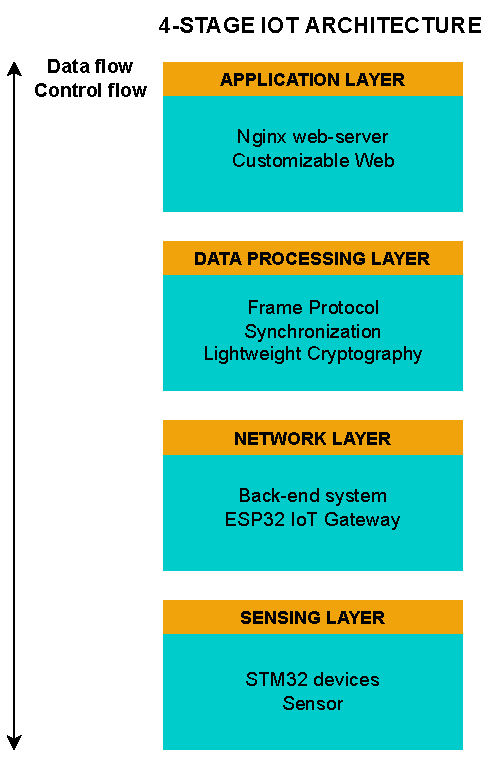
\includegraphics[width=8 cm]{images/Thesis-Page-2-IoT-Archi.pdf}
\caption{Mô hình 4 lớp của hệ thống IoT. Nguồn tham khảo InterviewBit~\cite{IoT-4-Layer-Archi}}
\label{fig:IoT-4-Layer-Archi-C2}
\end{figure}

\subsubsection{Sensing layer}

Đây là lớp đầu tiên của hệ thống \acrshort{iot} và sensing layer chứa các thiết bị vật lý, cảm biến, và ngoại vi trên bo mạch. Hoạt động của tầng này chủ yếu là thu thập và xử lý dữ liệu từ các cảm biến và ngoại vi, sau đó gửi dữ liệu lên tầng network.

Trong sensing layer, thiết bị sử dụng để giao tiếp với cảm biến và ngoại vi, là \acrshort{mcu} STM32. Các giao thức sử dụng trong tầng này là các giao thức có dây như UART, SPI, I2C,...

\subsubsection{Network layer}

Network layer là lớp chứa các thiết bị thu nhận và truyền tải dữ liệu trên Internet. Dựa trên lớp này, dữ liệu sẽ được luân chuyển từ \acrshort{iot} gateway đến các ứng dụng back-end.

Trong network layer, \acrshort{iot} gateway là \acrshort{mcu} ESP32 trên bo mạch. Gateway sẽ định tuyến dữ liệu từ hệ thống back-end đến sensing layer và ngược lại. Cuối cùng, hệ thống back-end thu nhận, xử lý, và lưu trữ dữ liệu từ sensing layer và đồng bộ các dữ liệu này với cơ sở dữ liệu của thiết bị vật lý và giao diện người dùng.

\subsubsection{Data processing layer}

Data processing layer là lớp chứa các kỹ thuật xử lý dữ liệu. Trong hệ thống này, data processing layer sẽ phân giải frame, mã hóa/giải mã dữ liệu, và đồng bộ dữ liệu với sensing và application layer.

\subsubsection{Application layer}

Application layer là lớp cung cấp ứng dụng của hệ thống thông qua các tương tác người dùng. Tại lớp này, hệ thống \acrshort{iot} sẽ cung cấp giao diện web tùy chỉnh cho người dùng. Từ đó, người dùng có thể giám sát và điều khiển dữ liệu của sensing và network layer.

\subsection{Giao thức frame}

\subsubsection{Tổng quan về giao thức frame}

Giao thức frame được định nghĩa để tạo ra cấu trúc frame trong giao tiếp device-gateway. Cấu trúc frame này là duy nhất và khác biết với các hệ thống khác. Điều này giúp việc giao tiếp trên bo mạch dễ triển khai và có tính bảo mật.

% Tại sao sử dụng gia thức frame
Trên bo mạch, giao thức frame giúp giao tiếp device-gateway có tính bảo mật và đáng tin cậy. Đầu tiên, hệ thống sẽ có cấu trúc frame duy nhất, riêng tư, và bảo mật. Vì vậy, cấu trúc frame này không thể phân giải trên các hệ thống khác. Tiếp theo, vì giao tiếp device-gateway có thể bị lỗi do nhiễu trên bo mạch, nên cấu trúc frame cung cấp các byte CRC để phát hiện lỗi khi giao tiếp diễn ra. Điều này đảm bảo hệ thống vẫn hoạt động khi gặp lỗi trong giao tiếp device-gateway.

% Cấu trúc frame
\subsubsection{Cấu trúc frame}

Cấu trúc frame (minh họa như hình \ref{fig:Frame-Structure-Overview}) được thiết kế bằng cách bố trí thêm các byte header, trailer, và CRC vào dữ liệu truyền. Cụ thể, headers chứa 2-byte h1 và h2; trailers chứa 2-byte t1 và t2; CRC chứa 2-byte CRC1 và CRC2 để tính toán CRC 16-bit; và phần body chứa 1-byte command, 2-byte data length, và các byte data.

% Ý nghĩa của các byte
Để nhận diện frame, các header và trailer dùng để nhận diện phần đầu và cuối frame. Tiếp theo, 1-byte command, 2-byte data length, và các byte data để hệ thống thực thi lệnh với dữ liệu tương ứng của frame. Cuối cùng, 2-byte CRC dùng để soát lỗi trên phần body của frame.

\begin{figure}[htp]
\centering
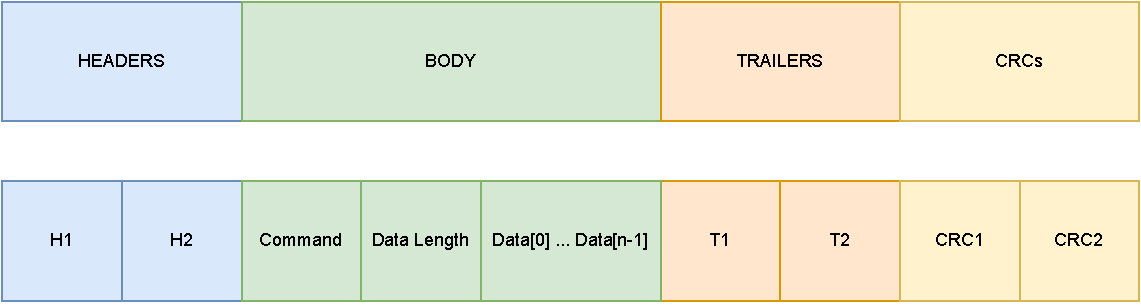
\includegraphics[width=0.9\linewidth]{images/Thesis-Page-4-Frame-Structure-Overview.pdf}
\caption{Cấu trúc frame của hệ thống.}
\label{fig:Frame-Structure-Overview}
\end{figure}

% Kỹ thuật phân giải frame

Để phân giải frame, kỹ thuật phân giải frame (minh họa như hình \ref{fig:frame-parsing-tech}) được triển khai trên giao tiếp UART của \acrshort{mcu} STM32 và gateway ESP32. Với mỗi byte nhận được, chỉ số của frame sẽ được kiểm tra. Với mỗi chỉ số frame, frame sẽ được kiểm tra header, trailer, CRC, hoặc thu thập các dữ liệu phần body. Cuối cùng, quá trình phần giải thành công khi việc tính toán CRC thành công và quá trình thất bại khi việc kiểm tra header, trailer, và CRC thất bại; hoặc timeout.

\begin{figure}[htp]
\centering
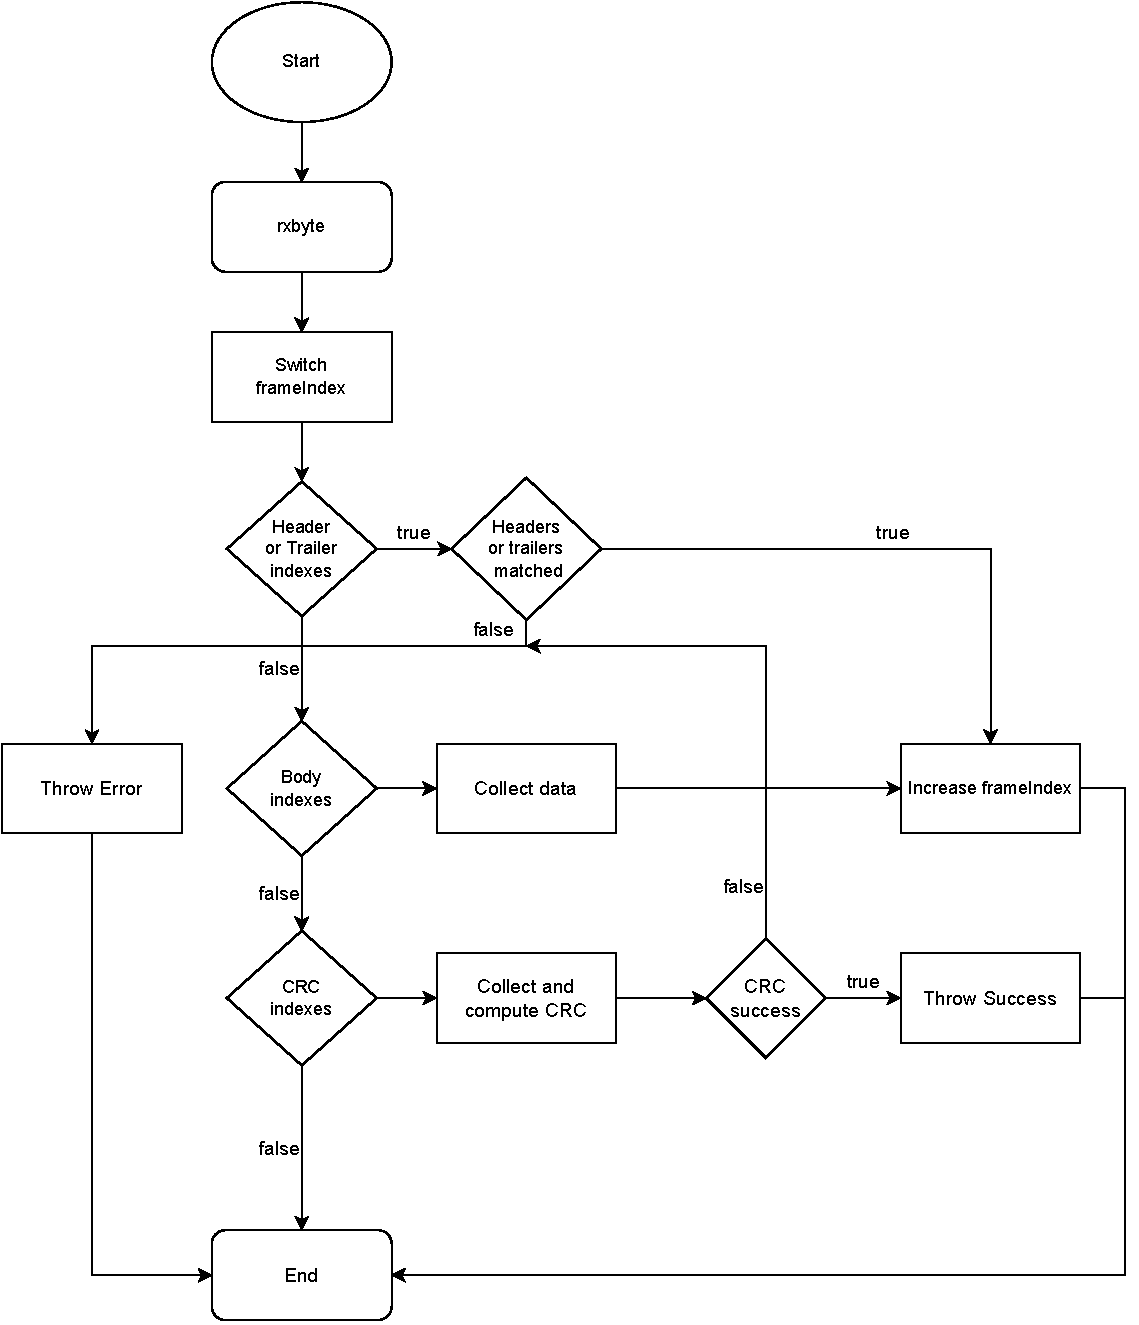
\includegraphics[width=1.0\linewidth]{images/Thesis-Page-5-Frame-Parsing-Tech.pdf}
\caption{Flowchart minh họa kỹ thuật phân giải frame.}
\label{fig:frame-parsing-tech}
\end{figure}

\subsection{Cơ chế đồng bộ}

% Vì sao cần cơ chế đồng bộ
Cơ chế đồng bộ (minh họa như hình \ref{fig:sync-mechani-overview}) được thiết kế dựa trên các yêu cầu cập nhật database. Với mỗi yêu cầu cập nhật dữ liệu của database, database phải thông báo sự kiện cập nhật tới \acrshort{api} server. Thông qua sự kiện cập nhật từ database, \acrshort{api} server sẽ đồng bộ dữ liệu được cập nhật với bo mạch và giao diện. Giao diện sẽ được đồng bộ trực tiếp qua Internet và thiết bị được đồng bộ gián tiếp qua \acrshort{iot} gateway.

\begin{figure}[htp]
\centering
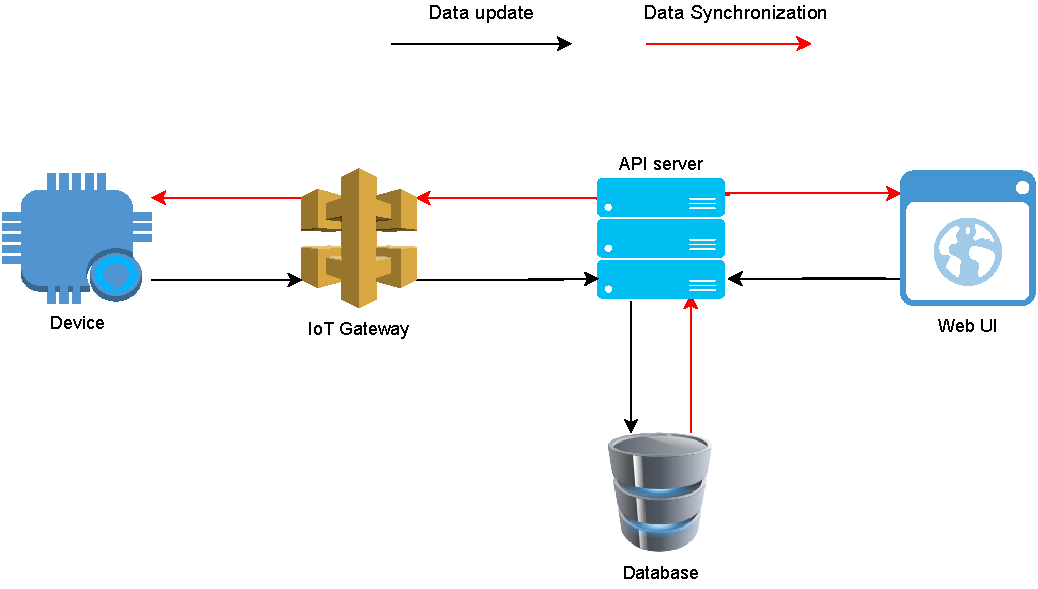
\includegraphics[width=1.0\linewidth]{images/Thesis-Page-6-sync-mecha.pdf}
\caption{Cơ chế đồng bộ của hệ thống \acrshort{iot}.}
\label{fig:sync-mechani-overview}
\end{figure}

\subsection{Giao diện web linh hoạt}

% Vì sao cần giao diện web linh hoạt
Trong các hệ thống \acrshort{iot}, cấu hình của các thiết bị luôn có thể thay đổi. Vì vậy, giao diện hiển thị cũng phải có tính linh hoạt và có thể tùy chỉnh để đáp ứng các thay đổi đó. Như vậy, giao diện có thể thay đổi tương ứng với cấu hình của các thiết bị. Hơn nữa, đối với người dùng, người dùng có thể dễ dàng thay đổi giao diện trong khi họ không cần phải lập trình.

% Cơ sở cho việc lập trình giao diện web linh hoạt
Giao diện web linh hoạt của hệ thống được phát triển trên framework ReactJS. Dựa trên framework này, thư viện ``React-Grid-Layout'' sẽ được sử dụng để phát triển giao diện linh hoạt. Khi sử dụng thu viện này, một hệ thống layout dạng lưới (minh họa như hình \ref{fig:RGL-overview}) sẽ được tạo ra. Trên mạng lưới đó, người dùng có thể kéo thả và thay đổi kích thước của các widget.

\begin{figure}[htp]
\centering
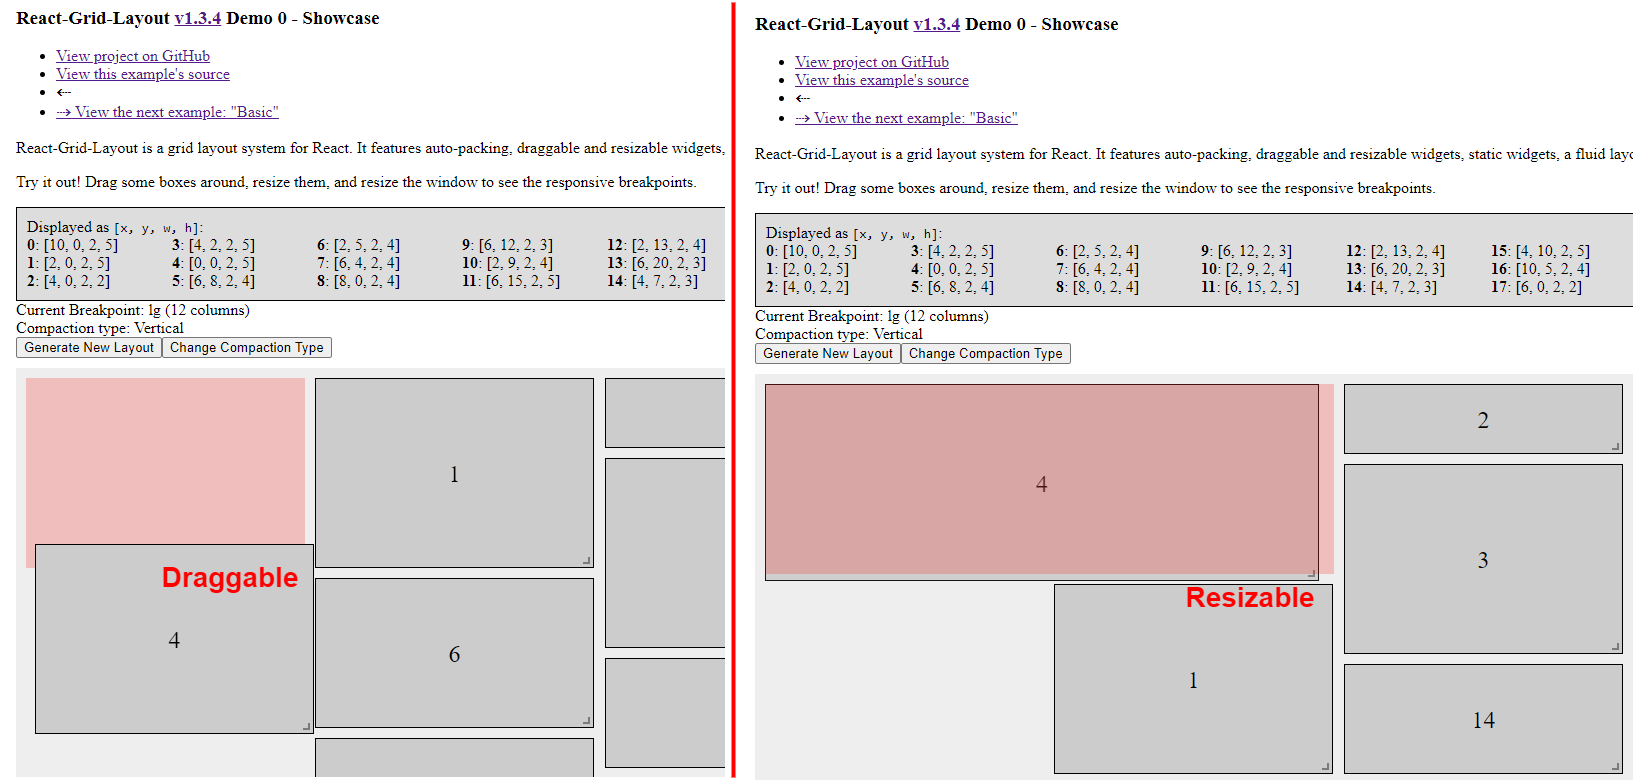
\includegraphics[width=1.0\linewidth]{images/Thesis-Page-7-RGL-Overview.png}
\caption{Hệ thống layout dạng lưới của React-Grid-Layout.}
\label{fig:RGL-overview}
\end{figure}

\subsection{Mật mã hóa nhẹ ChaCha20-Poly1305}

Mục này sẽ trích xuất và dịch thuật nội dung của RFC 7359~\cite{rfc7539}.

ChaCha20-Poly1305 là mật mã hóa xác thực với dữ liệu liên kết \acrfull{aead}. Đây là sự kết hợp của hai thuật toán độc lập. Thuật toán đầu tiên là ChaCha20, đây là thuật toán mã hóa dòng tốc độ cao. ChaCha20 được cho là nhanh hơn đáng kể so với thuật toán \acrfull{aes} trên môi trường software-only. Hơn nữa, ChaCha20 chạy nhanh hơn \acrshort{aes} ba lần trên những nền tảng không hỗ trợ phần cứng \acrshort{aes}. Về thuật toán Poly1305, Poly1305 là thuật toán xác thực tin nhắn tốc độ cao (high-speed message authentication code). Việc triển khai thuật toán này cũng rất dễ dàng và có độ chính xác cao.

\subsubsection{ChaCha Quarter Round}

Phép tính cơ bản của thuật toán ChaCha là quarter round. Nó tính toán dựa trên 4 số nguyên không dấu 32-bit, ký hiệu là a, b, c, và d. Việc tính toán diễn ra tuần tự như sau:

\begin{enumerate}
    \item a += b; d $\wedge$= a; d $<<<$= 16;
    \item c += d; b $\wedge$= c; b $<<<$= 12;
    \item a += b; d $\wedge$= a; d $<<<$= 8;
    \item c += d; b $\wedge$= c; b $<<<$= 7;
\end{enumerate}

Trong đó, dấu ``+'' ký hiệu cho phép cộng modulo 32-bit, ``$\wedge$'' ký hiệu cho toán tử bit \acrfull{xor}, và ``$<<<$ n'' ký hiệu cho n-bit dịch vòng bên trái (left rotation).

Về ChaCha state, ChaCha state là tập hợp của 16 số nguyên không dấu 32-bit, được biểu diễn dưới dạng ma trận 4x4 (như bảng \ref{tab:CC20-State-Pos}). Vì vậy, với mỗi phép toán quarter round, phép toán chỉ được thực hiện trên 4 trong số 16 số nguyên của ChaCha state.

\begin{table}[ht]
\caption{Mô tả bố cục ChaCha state ở dạng ma trận.}

\label{tab:CC20-State-Pos}%
\begin{center}
\begin{tabular}{|c|c|c|c|}
\hline
0  & 1  & 2  & 3  \\ \hline
4  & 5  & 6  & 7  \\ \hline
8  & 9  & 10 & 11 \\ \hline
12 & 13 & 14 & 15 \\ \hline
\end{tabular}
\end{center}
\end{table}

\subsubsection{ChaCha20 Block Function}

ChaCha20 Block Function là quá trình thực hiện việc biến đổi một ChaCha state bằng việc thực hiện nhiều lần các quarter round.

Đầu vào của khối ChaCha20 bao gồm:
\begin{itemize}
    \item Một key 256-bit, là sự kết hợp của 8 số nguyên 32-bit little-endian.
    \item Một nonce 96-bit, là sự kết hợp của 3 số nguyên 32-bit little-endian.
    \item Một khối đếm (block count parameter), là một số nguyên 32-bit little-endian.
\end{itemize}

Đầu ra của khối là 64 byte ngẫu nhiên.

Về việc khởi tạo ChaCha State, ChaCha State được khởi tạo bằng cách bố trí các tham số đầu vào của ChaCha20 dưới dạng ma trận 4x4 (minh họa như bảng \ref{tab:Init-CC20-State}) như sau:

\begin{itemize}
    \item 4 word đầu tiên (từ vị trí 0$\rightarrow$3) là các constant: 0x61707865, 0x3320646e, 0x79622d32, 0x6b206574.
    \item 8 word tiếp theo (từ vị trí 4$\rightarrow$11) được trích xuất từ 256-bit key bằng việc đọc các byte theo trật tự little-endian, đọc theo từng khối, mỗi khối là 1 word.
    \item Word thứ 12 là block counter. Vì mỗi ChaCha Block có độ dài 64 byte, một word 32-bit đủ cho 256 gigabytes dữ liệu. % 2^32 (bit) / 64(byte) = 256 ggByte
    \item Các word thứ 13$\rightarrow$15 là nonce, cùng một key thì không nên lặp lại nonce. Word thứ 13 là 32 bit đầu tiên của đầu vào nonce như một só nguyên little-endian, trong khi đó, word thứ 15 là 32 bit còn lại.
\end{itemize}

\begin{table}[ht]
\caption{Ma trận khởi tạo của ChaCha state.}

\label{tab:Init-CC20-State}%
\begin{center}
\begin{tabular}{|c|c|c|c|}
\hline
cccccccc & cccccccc & cccccccc & cccccccc \\ \hline
kkkkkkkk & kkkkkkkk & kkkkkkkk & kkkkkkkk \\ \hline
kkkkkkkk & kkkkkkkk & kkkkkkkk & kkkkkkkk \\ \hline
bbbbbbbb & nnnnnnnn & nnnnnnnn & nnnnnnnn \\ \hline
\end{tabular}
\end{center}
\end{table}

Trong đó, c=constant, k=key, b=blockcount, và n=nonce

Trong ChaCha20 Block Function, ChaCha20 chạy 20 round, xen kẽ giữa ``column rounds'' và ``diagonal rounds''. Mỗi round bao gồm bốn quarter-round, được minh họa như trình tự bên dưới. Trong một round của ChaCha20 Block Function, các quarter-round 1$\rightarrow$4 là phần thuộc ``column'' round, và 5$\rightarrow$8 là phần thuộc ``diagonal'' round:

\begin{enumerate}
    \item QUARTERROUND(0, 4, 8, 12)
    \item QUARTERROUND(1, 5, 9, 13)
    \item QUARTERROUND(2, 6, 10, 14)
    \item QUARTERROUND(3, 7, 11, 15)
    \item QUARTERROUND(0, 5, 10, 15)
    \item QUARTERROUND(1, 6, 11, 12)
    \item QUARTERROUND(2, 7, 8, 13)
    \item QUARTERROUND(3, 4, 9, 14)
\end{enumerate}

Sau khi kết thúc 20 round (hoặc 10 lần thực hiện 8 trình tự ở trên), các word đầu vào ban đầu được cộng với các word đầu ra. Sau đó, kết qua được serialize bằng việc sắp xếp các từng word một theo trình tự little-endian.

\subsubsection{Thuật toán mã hóa ChaCha20}

ChaCha20 là mã hóa dòng được thiết kế bởi D. J. Bernstein. Nó là sự cải tiến của thuật toán Salsa20, và sử dụng 256-bit key.

ChaCha20 liên tục thực thi ChaCha20 Block Function, với cùng key và nonce, và với việc liên tục tăng block counter. Sau đó, ChaCha20 sẽ tuần tự hóa (serialize) kết quả của ChaCha state bằng việc ghi các số theo thứ tự little-endian, tạo keystream block.

Đầu vào của thuật toán ChaCha20 bao gồm
\begin{itemize}
    \item Một key 256-bit.
    \item Một counter 32-bit ban đầu. Counter có thể thiết lập bất cứ giá trị nào, nhưng thường là 0 hoặc 1. Điều này có nghĩa khi dùng một lần nếu ta sử dụng khối couter 0 cho việc gì đó, ví dụ như việc tạo ra one-time authenticator key như là một phần của thuật toán \acrshort{aead}.
    \item Một nonce 96-bit. Trong một số giao thức, nonce được xem như là một vector khởi tạo.
    \item Một plaintext có độ dài tùy ý.
\end{itemize}

Đầu ra của thuật toán là tin nhắn được mã hóa, hoặc ``ciphertext'', có cùng độ dài.

Việc giải mã được tiện hành tương tự như mã hóa. ChaCha20 Block Function được sử dụng để tạo keystream, nó được dùng để \acrshort{xor} với ciphertext để khôi phục lại plaintext.

\subsubsection{Thuật toán Poly1305}
\label{Poly1305Algorithm}

Poly1305 là thuật toán tạo xác thực một lần (one-time authenticator) được thiết kế bởi D. J. Bernstein. Poly1305 dùng 32-byte one-time key và một message, và cho ra một xác thực 16-byte tag. Tag này dùng để xác thực message.

Bất kể key được tạo ra như thế nào, key được phân vùng thành hai phần, được gọi là ``r'' và ``s''. Cặp (r,s) nên là duy nhất, và bắt buộc không thể dự đoán trước trong mỗi lần tạo, ``r'' có thể tùy chỉnh là một hằng số.

``s'' nên được tạo ra có tính chất không thể dự đoán trước, nhưng hoàn toàn chấp nhận việc tạo ra cả ``r'' và ``s'' một cách duy nhất tại một thời điểm. Bởi vì cả ``r'' và ``s'' đều có độ dài 128 bit, nên tạo ra chúng một cách ngẫu nhiên thì cũng chấp nhận được.

Đầu vào của thuật toán Poly1305 bao gồm:

\begin{itemize}
    \item Một one-time key 256-bit.
    \item Một message có độ dài tùy ý.
\end{itemize}

Đầu ra của thuật toán là 128-bit tag.

Thuật toán Poly1305 diễn ra tuần tự như sau. Đầu tiên, giá trị của ``r'' được kẹp chặt (clamp).

Tiếp đến, thiết lập hằng số nguyên số ``P'' là $2^{135}$ – 5: 3fffffffffffffffffffffffffffffffb. Sau đó ta cũng thiết lập biến ``accumulator'' bằng 0.

Sau đó, chia message thành các khối 16-byte. Khối cuối cùng có thể có độ dài ngắn hơn:

\begin{itemize}
    \item Đọc khối message như từng số little-endian.
    \item Thêm một bit ở vị trí ngoài cùng của các octet. Với một khối 16-byte, điều này tương đương với việc cộng với $2^{128}$. Khối có độ dài nhỏ hơn 10-byte, nó có thể là $2^{120}$, $2^{112}$, hoặc bất cứ số là lũy thừa của 2 mà nó có thể chia hết cho 8, nhỏ nhất là $2^8$.
    \item Nếu block không có độ dài 17 byte (ở block cuối cùng), thêm các bit 0 (pad) vào block. Điều này là vô nghĩa nếu ta coi các block như các số nguyên.
    \item Cộng số này với ``accumulator''.
    \item Nhân ``accumulator'' với ``r''.
    \item Thiết lập ``accumulator'' bằng phép chia modulo cho ``P''. \\Tóm lại: $accumumator = ((accumulator+block)*r) \% P$.
\end{itemize}

Cuối cùng, giá trị của secret key (``s'') được cộng vào ``accumulator,  và 128 least significant bit được tuần tự hóa theo trật tự little-endian.

\subsubsection{Tạo Poly1305 key sử dụng ChaCha20}
\label{CreatePoly1305UsingChaCha20}

Như đã đề cập ở mục \ref{Poly1305Algorithm}, có thể chập nhận việc tạo one-time key cho Poly1305 một cách giả ngẫu nhiên (pseudorandomly). Ở mục này, phương pháp được đề xuất là tạo one-time key cho Poly1305 sử dụng ChaCha20.

Để tạo cặp key (r,s), chúng ta sử dụng ChaCha20 Block Function. Phương pháp được đề xuất là gọi ChaCha20 Block Function với các tham số đầu vào như sau:

\begin{itemize}
    \item 256-bit key từ keystream sinh ra từ ChaCha20 Block Function.
    \item Block counter thiết lập bằng 0.
    \item Một nonce 96-bit.
\end{itemize}

Sau khi chạy ChaCha20 Block Function, nó sinh ra 512-bit state. Lấy 256 bit đầu tiên hoặc state tuần tự hóa (serialized state), và sử dụng chúng như one-time Poly1305 key: 128 bit đầu tiên giữ lại và hình thành nên ``r'', và 128 bit còn lại trở thành ``s''. 256 bit còn lại bị loại bỏ.

\subsubsection{Cấu trúc AEAD}

Cấu trúc \acrshort{aead} cho thuật toán ChaCha20-Poly1305 là mã hóa xác thực với dữ liệu liên kết. Các input cho AEAD\_CHACHA20\_POLY1305 là:

\begin{itemize}
    \item Một key 256-bit.
    \item Một nonce 96-bit.
    \item Một plaintext có độ dài tùy ý.
    \item Dữ liệu xác thực liên kết với độ dài tùy ý - \acrfull{aad}.
\end{itemize}

Các thuật toán gốc của ChaCha20 và Poly1305 được kết hợp thành \acrshort{aad} có đầu vào là một key 256-bit và nonce 96-bit như sau:

\begin{itemize}
    \item Đầu tiên, Poly1305 one-time key được tạo ra từ key 256-bit và nonce sử dụng phương pháp ở mục \ref{CreatePoly1305UsingChaCha20}.
    \item Tiếp theo, function, thực hiện mã hóa ChaCha20, được thực thi để mã hóa plaintext, sử dụng cùng key và nonce, và với couter được thiết lập bằng 1.
    \item Cuối cùng, Poly1305 function được thực thi với đầu vào là Poly1305 key được tính toán ở trên, và một message (plaintext).
\end{itemize}

Output từ \acrshort{aead} là hai thành phần sau:
\begin{itemize}
    \item Một ciphertext có cùng độ dài với plaintext.
    \item Một tag 128-bit, là output của Poly1305 function.
\end{itemize}

Việc giải mã là tương tự với những khác biệt sau:
\begin{itemize}
    \item Các vai trò của ciphertext và plaintext được hoán đổi, nên function mã hóa ChaCha20 được áp dụng cho ciphertext, cung cấp plaintext.
    \item Poly1305 function vẫn thực thi dựa trên \acrshort{aad} và cipher text, không phải plaintext.
    \item Tag được tạo ra, được so sánh tag nhận được. Message được xác thực khi và chỉ khi các tag trùng khớp với nhau.
\end{itemize}